\section{ML Model Methodology}
This section provides a comprehensive overview of the methodologies employed in the construction of the machine
learning model. The discussion encompasses various techniques designed to handle the intricacies of model building,
coupled with a logical flow that guides the entire process.

% ------------------- Data Preparation -------------------

\subsection{Preliminary Data Preparation}\label{subsec:preliminary_data_preparation}
Before delving into model development, a data preprocessing pipeline was employed to properly prepare them for the subsequent steps, facing the problems
of class imbalance and training computational complexity.\\
\begin{itemize}
	\setlength\itemsep{1em} % set space between items
	\item \textbf{Random Sampling}: Given the extensive nature of hyperparameter tuning, we adopted a random sampling strategy, picking around 10\% of the dataset.
	      Instead of training the models on the entire dataset for each hyperparameter combination, the random subset was used to expedite the tuning
	      phase without sacrificing model representativity.
	\item \textbf{Class Imbalance with Oversampling and Undersampling}: The dataset was highly unbalanced across its 700 disease classes.
	      To mitigate this, a combination of oversampling and undersampling techniques was applied. The former was performed for minority classes,
	      while the latter was applied to the majority classes, ensuring all the diseases were adequately represented during training,
	      preventing dominance and biases in the model.
\end{itemize}


% ------------------- Feature Extraction -------------------

\subsection{Feature Extraction}
% - Prepare the features and normalization
A pivotal phase in constructing a machine learning model is feature extraction. In addition to the one-hot vector representation
of symptoms, the network analysis affords us the following features:\\

\begin{itemize}
	\setlength\itemsep{1em} % set space between items
	\item \textbf{L1 and L2 Measures}: A vector with values representing the L1 and L2 measures for each symptom.
	\item \textbf{Betweenness Centrality}: A vector with values denoting the betweenness centrality of each symptom.
	\item \textbf{Community Count}: A vector indicating the number of symptoms belonging to each community.
	\item \textbf{Community Size}: A vector replacing symptoms with the size of the community to which they belong.
\end{itemize}
\noindent
Given the diverse scales of these features, normalization becomes imperative for their cohesive integration into the model
without introducing biases. To achieve this, we opted for \textit{MaxAbs} normalization. This normalization scales each feature
individually, ensuring that the maximal absolute value of each feature in the training set becomes 1.0, while preserving the sparsity of data.


% ------------------- Model Choice -------------------

\subsection{Model Choice}

In the expansive landscape of machine learning, numerous classification models are available for disease prediction.
Our selection narrows down to three models renowned for their robust predictive capabilities,
as substantiated by the findings of \citeauthor{Kohli}~\cite{Kohli}, \citeauthor{Singh}~\cite{Singh}, and \citeauthor{Uddin2019Dec}~\cite{Uddin2019Dec}.
These models are Logistic Regression, Random Forest, and Multilayer Perceptron (MLP).\\


\noindent
\textbf{Logistic Regression}\vspace{0.15cm}
\begin{itemize}
	\item \textbf{Strengths}: Logistic Regression's computational efficiency makes it an attractive choice for initial exploration and
	      baseline performance assessment. Its simplicity facilitates interpretability, providing insights into the impact of individual symptoms on disease prediction.
	\item \textbf{Considerations}: While efficient, Logistic Regression assumes a linear relationship between features and the
	      log-odds of the target, potentially limiting its ability to capture complex non-linear patterns.
\end{itemize}

\noindent
\textbf{Random Forest}\vspace{0.15cm}
\begin{itemize}
	\item \textbf{Strengths}: Random Forest is renowned for its robustness in handling large and diverse datasets, making
	      it well-suited for our expansive dataset with 700 disease classes. Moreover, Its ability to capture non-linear relationships
	      ensures that complex patterns within the symptoms' one-hot encoded features are effectively modeled.
	\item \textbf{Considerations}: The ensemble nature of Random Forest provides resilience against overfitting, a crucial factor
	      in the context of disease prediction.
\end{itemize}

\noindent
\textbf{Multilayer Perceptron (MLP)}\vspace{0.15cm}
\begin{itemize}
	\item \textbf{Strengths}: MLPs are adept at capturing intricate relationships in high-dimensional datasets,
	      aligning with the complexity inherent in our 300-feature symptom representation.
	\item \textbf{Considerations}: Their capacity for adapting to non-linear mappings positions MLPs as powerful
	      tools in unraveling the nuanced interactions between symptoms and diseases.
\end{itemize}



% ------------------- Operative Flow -------------------

\subsection{Operative Flow}
% - Operative Flow
% - select best parameters for symptoms one hot only
% - select best parameters for combination of other features (best combination is chosen with random parameters looking at the accuracy)
% - train for each model the two version above with optimal parameters
% - pick the best model according to accuracy
% - train the best model with whole dataset and reduce the number of features

\begin{figure}[t]
	\centering
	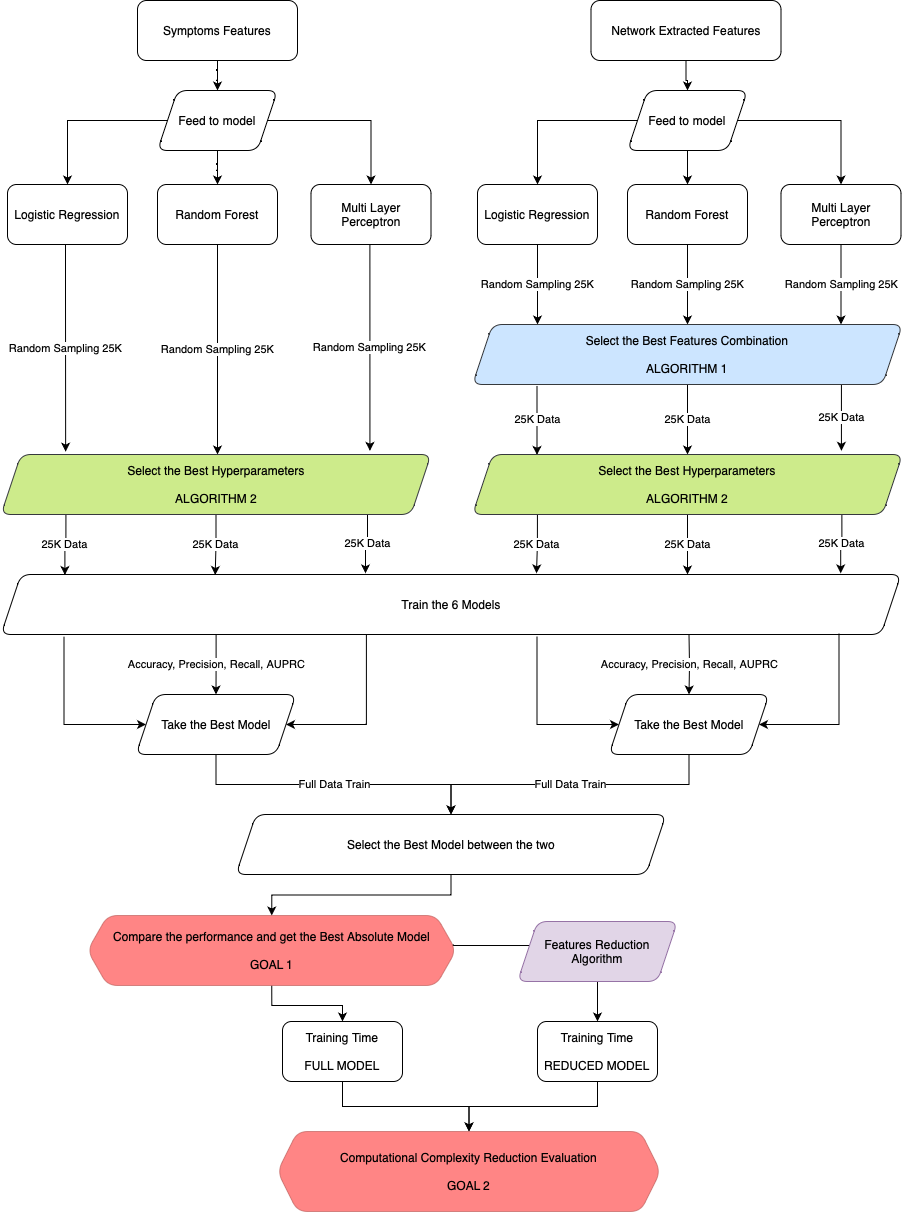
\includegraphics[width=\columnwidth]{operational_flow.png}
	\caption{Operative Flow of the ML Model}\label{fig:ML_operative_flow}
\end{figure}

Once the features are ready, the core part of the model-building process can begin. The operational flow was quite complex,
and it is summarized in Figure~\ref{fig:ML_operative_flow}.\\
We trained three different models: a Logistic Regression, a Random Forest, and a Multi-Layer Perceptron (MLP).\\
For each model, we faced the challenge of selecting both the best hyperparameters and the most effective features.
The interdependence between these two aspects makes the optimal approach to explore all the possible combination of features
and for each combination trying all the hyperparameters combination. This approach is not feasible in terms of computational effort
leading us to adopt a greedy approach. We firstly split the features into two
groups: the symptoms' one-hot vector and the remaining features. The former is used to train a base model,
while the latter is utilized to explore the potential improvement brought by the new features.\\
Using Algorithm~\ref{alg:feature_selection}, we determined the best feature combination for each group (symptoms and other features).
Subsequently, given the optimal feature combination, we identified the best Hyperparameters combination using Algorithm
~\ref{alg:greedy_hyperparameter_search}. Each model was then trained with the best hyperparameters and the best features combination.
For each group of three models available at this point (3 models with symptoms and 3 models with other features), we selected the best one
according to their accuracy value (Section~\ref{subsubsec:results_ML_model_comparison}).
Only at this point the two winning models were trained with the whole dataset to provide a more precise evaluation of their performance and
were compared to assess the result of our first Goal.\\
As regard the last Goal, the best between the above two models undergone the feature reduction process
discussed in Section~\ref{subsec:most_important_actors} and its computational time was compared to the one of the full features model.\\

\begin{algorithm}[t] \small
	\caption{Feature Selection Algorithm}\label{alg:feature_selection}

	\begin{algorithmic}[1]
		\State RemainingFeatures $\gets$ AllFeatures
		\State FeatureSet $\gets$ EmptySet
		\State BestAccuracies $\gets$ EmptySet
		\State Parameters $\gets$ InitializeRandomParameters
		\State i $\gets$ 0

		\While{RemainingFeatures is not Empty}
		\State BestAccuracy $\gets$ 0

		\For{each feature in RemainingFeatures}
		\State CurrentFeatureSet $\gets$ feature $\cup$ FeatureSet
		\State Model $\gets$ EmptyModel
		\State TrainModel(odel, CurrentFeatureSet, Parameters)
		\State CurrentAccuracy $\gets$ GetAccuracy(Model)

		\If{CurrentAccuracy $>=$ BestAccuracy}
		\State BestAccuracy $\gets$ CurrentAccuracy
		\State BestFeature $\gets$ feature
		\EndIf
		\EndFor

		\State BestAccuracies[i] $\gets$ BestAccuracy
		\State RemainingFeatures $\gets$ RemainingFeatures $-$ BestFeature
		\State FeatureSet $\gets$ BestFeature $\cup$ FeatureSet
		\State BestFeatureCombinations[i] $\gets$ FeatureSet
		\State i $\gets$ i $+$ 1
		\EndWhile
		\State BFC $\gets$ BestFeatureCombinations[ArgMax(BestAccuracies)]
		\State \textbf{return} BFC

	\end{algorithmic}
\end{algorithm}

The quest for optimal hyperparameters (hparams) in machine learning models is often constrained by computational resources. In light of these
limitations, we adopted a resource-efficient greedy search strategy to navigate the vast hyperparameter space.
Our approach unfolds in several stages. Initially, we randomly initialize hyperparameters (hparams) to initiate the search. Subsequently, we employ
a stepwise exploration, beginning with the first hyperparameter. For this, we perform an initial search over a small set of values
(e.g., 0.001, 0.01, 1, 10, 100). If the optimum lies at one of the extremes, we extend the search to encompass values in the corresponding
direction.; conversely, if it resides within an intermediate range, we conduct a more focused exploration in a narrower interval.
This process is iteratively repeated for each hyperparameter, gradually refining our understanding of the optimal regions within the
hyperparameter space.
This iterative approach serves a dual purpose. First, it conserves computational resources by avoiding an exhaustive search over all
potential combinations. Second, it capitalizes on the information gleaned from earlier iterations to guide subsequent searches efficiently.
By strategically determining the next set of values based on the observed trends, we strike a balance between exploration and exploitation,
ultimately converging to a set of hyperparameters (hparams) that maximizes model performance. This resource-conscious strategy is paramount when
computational resources are limited, allowing us to derive meaningful results within practical constraints.

% TO BE MODIFIED BY CRISTIAN
\begin{algorithm}[H]
	\caption{Greedy Hyperparameter Search}\label{alg:greedy_hyperparameter_search}
	\begin{algorithmic}[1]
		\State hparams $\gets$ randomInitialization

		\For{each hparam in hparams}
		\State src\_range $\gets$ initialSrcRange
		\State best\_value $\gets$ curr\_hparams[hparam]
		\State accuracy $\gets$ 0

		\For{value in src\_range}
		\State curr\_hparams[hparam] $\gets$ value
		\State performance $\gets$ eval(model, curr\_hparams)

		\If{performance better than accuracy}
		\State best\_value $\gets$ value
		\State accuracy $\gets$ performance
		\EndIf
		\EndFor

		\If{best\_value is at the lower extreme}
		\State src\_range $\gets$ extendSrcRangeLower(best\_value)
		\ElsIf{best\_value is at the upper extreme}
		\State src\_range $\gets$ extendSrcRangeUpper(best\_value)
		\Else
		\State src\_range $\gets$ narrowSrcRange(best\_value)
		\EndIf

		\For{value in src\_range}
		\State curr\_hparams[hparam] $\gets$ value
		\State performance $\gets$ eval(model, curr\_hparams)

		\If{performance better than accuracy}
		\State best\_value $\gets$ value
		\State accuracy $\gets$ performance
		\EndIf
		\EndFor
		\State curr\_hparams[hparam] $\gets$ best\_value
		\EndFor
	\end{algorithmic}
\end{algorithm}
\noindent

At the conclusion of these procedures, we obtained the following two models:\\

\begin{itemize}
	\setlength\itemsep{0.4em} % set space between items
	\item \textbf{Symptoms Model}: The best model with the optimal hparams and the symptoms as features
	\item \textbf{Other Features Model}: The best model with the optimal hyperparameters and the best features combination
\end{itemize}
\vspace{0.4cm}

